\section{Experiments}
%\subsection{Datasets \& Implementation Details}
\noindent
\textbf{Datasets.}
We conduct our experiments on ScanNetV2 \cite{scannet} and 7Scenes datasets \cite{7scenes}  for training and evaluation. ScanNet is a real dataset for indoor 3DR, which consists of 2.5M images captured in 1513 different indoor scenes. 7Scenes is another challenging indoor real dataset, consisting of  7 scenes, with rich contents of RGB, depth, and camera pose.

\noindent
\textbf{Metrics.}
We use the same evaluation metrics as Atlas \cite{atlas} and NeuralRecon \cite{neucon}, and we evaluate both 3D geometric mesh metrics and 2D rendered depth metrics. As in \cite{atlas}, since there is no depth directly estimated from the model, we project 3D mesh to get 2D depth maps and use the rendered depth maps for 2D metrics evaluation.

\noindent
\textbf{Implementation Details.}
The weights for each loss ``$\lambda_{sdf}$, $\lambda_{plane}$, $\lambda_{depth}$, $\lambda_{NeRF}$'' are ``1, 0.05, 1, 1'', respectively. For fair comparison with previous voxel-SDF works, we use the same voxel configurations where voxel size is set to $4cm$, scene fragment resolution is set to $96\times96\times96$, SDF truncation distance is set to $30cm$, max depth for ground truth SDF fusion is set to $3m$. We train and test on all samples based on standard training/testing splits of ScanNet where entire framework is trained end-to-end in pure self-supervision from scratch with randomly initialized weights, except for the image encoder Resnet-18, which we choose to be light and efficient. We train on randomly separated scene fragments over all scenes for the first 20 epochs without GRU, which is to reinforce the inner-consistency within fragments and warmup for each part of the framework. We then train on each continuous scene fragments over all scenes together with GRU to reinforce the inter-consistency between fragment. We use 7Scenes only for few-shot transfer and testing. We use NeRF decoder only in training to boost SDF estimation, and we only keep SDF for testing and inference. 

\subsection{Evaluation Results}
\noindent
\textbf{Baselines.} We conduct evaluation and comparison with monocular 3DR in Table \ref{table:3dr class}. Although non-generalizable methods\cite{neuralangelo,neuralwarp,neuris} generate accurate results, they train with one scene and can be only tested on the same scene, which is under completely different training/testing setup to ours, so we do not directly compare with these works. For the generalizable supervised voxel-SDF methods \cite{atlas,neucon}, we directly compare both 3D geometric mesh and 2D rendered depth. Since we get 3D mesh ground truth by fusing SDF with depth map ground truth, to make the comparison rigorous and fair, we get estimated 3D mesh by fusing SDF with estimated depth from self-supervised/supervised depth estimation works. For supervised depth methods \cite{mvdepthnet, gpmvs, dpsnet}, we directly use their depth estimation for SDF fusion, for self-supervised depth \cite{p2net, monoindoor, movingindoor, structdepth}, and since there is scale ambiguity, we first use ground truth depth to recover real scale for estimated depth, and then fuse SDF. NYUV2 is the most popular dataset for indoor depth estimation. Since our SDF regression requires camera pose and NYUV2 does not offer it, we do not test on NYUV2. However, we choose the currently best three self-supervised models \cite{distdepth, structdepth, p2net} from NYUV2 leaderboard for comparison. Although trained on NYUV2, these models claim zero-shot transfer for indoor scenes by testing a subset of ScanNet in their original papers. We test them with the full testing split for comparison with our work. MonoNeRF \cite{mononerf} is our strongest baseline, which also uses the same training/testing splits of ScanNet as in our method. It is the latest self-supervised work to jointly train NeRF with a SFM model, and use NeRF to boost SFM performance.  Our self-supervised voxel-SDF regression is also based on SFM, but MonoNeRF is still depth estimation while our MonoSelfRecon estimates continuous 3D mesh for a whole scene. 

\begin{table}[]
%\resizebox{\textwidth}{!}
\setlength\tabcolsep{1pt}
\footnotesize
\begin{tabular}{llllllll}
\hline
\textbf{2D Depth}         & Train        & AbsRel$\downarrow$ & AbsDiff$\downarrow$ & SqRel$\downarrow$ & RMSE$\downarrow$  & \textbf{$\delta1\uparrow$}  & Comp$\uparrow$  \\ \hline
MVDepthNet\cite{mvdepthnet}     & sup         & 0.098   & 0.191    & 0.061  & 0.293 & 89.6 &  0.928 \\
GPMVS\cite{gpmvs}          & sup          & 0.130   & 0.239    & 0.339  & 0.472 & 90.6 & 0.928 \\
DPSNet\cite{dpsnet}         & sup          & 0.087   & 0.158    & 0.035  & 0.232 & 92.5 & 0.928 \\
COLMAP\cite{colmap}         & sup          & 0.137   & 0.264    & 0.138  & 0.502 & 83.4 & 0.871 \\
Atlas\cite{atlas}          & sup          & 0.065   & 0.123    & 0.045  & 0.251 & 93.6 & 0.999 \\
NeuralRecon\cite{neucon}    & sup          & 0.065   & 0.106    & 0.031  & 0.195 & 94.8 & 0.909 \\
NeuralRecon\cite{neucon}    & weak         & 0.107   & 0.183    & 0.046  & 0.268 & 87.2 & 0.817 \\
\hline
Distdepth\cite{distdepth}   & self      & 0.360   & 0.485    & 0.308  & 0.583 & 48.0 & 0.889 \\
Monodepth2\cite{monodepth2}   & self      & 0.205   & -    & 0.129  & 0.453 & 67.9 & - \\
P2Net\cite{p2net}   & self               & 0.253   & 0.336    & 0.171  & 0.429 & 65.1 & 0.888 \\
Structdepth\cite{structdepth}   & self      & 0.219   & 0.139    & 0.139  & 0.383 & 70.9 & 0.896 \\
MonoNeRF\cite{mononerf}   & self         & 0.169   & -    & 0.089  & 0.375 & 76.0 & - \\
Ours  & self                    &0.143    & 0.231    & 0.090  & 0.333 & 79.2 & 0.872 \\
Ours  & weak                    &0.089    & 0.134    & 0.038  & 0.208 & 89.8 & 0.827 \\\hline
\end{tabular}
\setlength\tabcolsep{3.5pt}
\begin{tabular}{lllllll}
\textbf{3D Mesh}         & Train        & Comp$\downarrow$  & Acc$\downarrow$   & Recall$\uparrow$ & Prec$\uparrow$  & \textbf{F-score$\uparrow$} \\ \hline
MVDepthNet\cite{mvdepthnet}     & sup        & 0.040 & 0.240 & 0.831  & 0.208 & 0.329   \\
GPMVS\cite{gpmvs}          & sup         & 0.031 & 0.879 & 0.871  & 0.188 & 0.304   \\
DPSNet\cite{dpsnet}         & sup         & 0.045 & 0.284 & 0.793  & 0.223 & 0.344   \\
COLMAP\cite{colmap}         & sup         & 0.069 & 0.135 & 0.634  & 0.505 & 0.558   \\
Atlas\cite{atlas}          & sup         & 0.062 & 0.128 & 0.732  & 0.382 & 0.499   \\
NeuralRecon\cite{neucon}    & sup         & 0.120 & 0.062 & 0.428  & 0.592 & 0.494   \\
NeuralRecon\cite{neucon}    & weak         & 0.262 & 0.089 & 0.157  & 0.308 & 0.205   \\
\hline
Distdepth\cite{distdepth}   & self   & 0.262 & 0.371 & 0.159  & 0.104 & 0.121    \\ 
P2Net\cite{p2net}   & self  & 0.170 & 0.264 & 0.231  & 0.148 & 0.179    \\ 
Structdepth\cite{structdepth}   & self      & 0.170 & 0.217 & 0.243  & 0.181 & 0.207    \\ 
Ours   & self                   & 0.212 & 0.185 & 0.262  & 0.263 & 0.260    \\ 
Ours   & weak                   & 0.197 & 0.075 & 0.293  & 0.469 & 0.358    \\ \hline
\end{tabular}
\vspace{-3mm}
\caption{\textbf{2D Depth and 3D Mesh metrics on ScanNet.} ``sup'' ``self'' ``weak'' denote supervised, self-supervised, and weakly supervised training, respectively. We use the same training/testing splits as \cite{atlas, neucon}, where the results of \cite{mvdepthnet,gpmvs,dpsnet,colmap} are directly from \cite{atlas, neucon}'s papers, and we test \cite{distdepth,p2net,structdepth} in this work. Results of \cite{monodepth2, mononerf} are directly from \cite{mononerf} since it also uses same training/testing splits as \cite{atlas,neucon} and our method. Since MonoNeRF\cite{mononerf}'s code is not released, 3D mesh of \cite{mononerf,monodepth2} from Table \ref{table:scannet} are not available, so they are not compared in this table.
}
\label{table:scannet}
\vspace{-7mm}
\end{table}


\noindent
\textbf{ScanNet.} For depth evaluation, we follow the same standards of previous works \cite{atlas, neucon} to render depth from 3D mesh. Table \ref{table:scannet} shows both rendered 2D depth and 3D mesh comparison. Our MonoSelfRecon outperforms all SOTA self-supervised depth estimation from NYUV2 leaderboard, especially the latest strongest baseline MonoNeRF. The 3D mesh comparison shows consistent results to 2D rendered depth. Since MonoNeRF has not released their code, we only compare it for 2D depth and could not generate their 3D mesh for comparison. 

Although our MonoSelfRecon outperforms all SOTA generalizable self-supervised 3DR and is comparable to depth-based purely-supervised 3DR, there is still a clear gap to purely-supervised voxel-SDF methods using fine-grained SDF annotations, so we conduct experiments on weakly-supervised training to further demonstrate our design. While all supervised voxel-SDF methods \cite{atlas,neucon,vortx} use voxel-SDF annotations for a L1 loss, NeuralRecon also uses a coarse binary voxel-mask annotations as weakly supervised signal, where the mask tells if each voxel-SDF is within truncation distance. In our purely self-supervised model setup, we filter out invalid voxels beyond truncation distance at each level of the SDF decoder in both training and testing, and only pass valid voxels to the next level. While for our weakly-supervised training, inspired by NeuralRecon, besides using our self-supervised losses, we add a mask regressor at each level and supervise with coarse mask ground truth, which is only used for training, and the mask regressor estimates valid voxels in testing. As Table \ref{table:scannet} shows, our model improves obviously with coarse mask signal, and is even better than some fully-supervised works. More importantly, we also conduct weakly-supervised training by removing SDF ground truth and only using mask for original NeuralRecon, and we train both works to same epochs. Comparing weakly-supervised results, we clearly outperform NeuralRecon in weak supervision, which validates our purely self-supervised design.

\begin{table}[]
%\small
\footnotesize
\setlength\tabcolsep{2pt}
\begin{tabular}{lllllll}
\hline
\textbf{2D Depth}        & Train    & \textbf{$\delta1\uparrow$}     & AbsRel$\downarrow$ & SqRel$\downarrow$ & RMSE$\downarrow$ & Comp$\uparrow$\\ \hline
DeMoN\cite{demon}   & sup   & 31.9 & 0.389 & 0.420  & 0.855 & -    \\ 
MVSNet\cite{mvsnet}   & sup  & 64.1 & 0.234 & 0.190  & 0.508 & -    \\ 
NeuralRGBD\cite{neuralrgb}   & sup      & 69.3 & 0.176 & 0.112  & 0.440 & -    \\ 
MVDNet\cite{mvdepthnet}   & sup     & 71.8 & 0.193 & 0.235  & 0.459 & -    \\ 
DPSNet\cite{dpsnet}   & sup      & 70.9 & 0.199 & 0.142  & 0.438 & -    \\ 
DeepV2D\cite{deepv2d}     & sup        & 42.8  & 0.437 & 0.553  & 0.869 & -   \\
CNMNet\cite{CNMNet}          & sup         & 76.6 & 0.161 & 0.083  & 0.361 & -   \\
NeuralRecon\cite{neucon}    & sup         & 82.0 & 0.155 & 0.104  & 0.346 & -   \\
Neucon\_weak\cite{neucon}    & weak         & 78.2 & 0.163 & 0.101  & 0.303 & 0.626   \\
Ours(weak)   & weak                   & 68.0 & 0.209 & 0.148  & 0.474 & 0.634    \\ 
Ours(self)   & self                   & 63.3 & 0.219 & 0.155  & 0.519 & 0.818    \\ \hline
\textbf{3D Mesh}         & Train        & \textbf{F-score$\uparrow$}  & Recall$\uparrow$ & Prec$\uparrow$  &  Comp$\downarrow$ & Acc$\downarrow$\\ \hline
DeepV2D\cite{deepv2d}     & sup        & 0.115 & 0.175 & 0.087  & 0.180 & 0.518   \\
CNMNet\cite{CNMNet}          & sup         & 0.149 & 0.246 & 0.111  & 0.150 & 0.398   \\
NeuralRecon\cite{neucon}    & sup         & 0.282 & 0.227 & 0.389  & 0.228 & 0.100   \\
Neucon\_weak\cite{neucon}    & weak         & 0.101 & 0.062 & 0.356  & 0.103 & 0.473   \\
Ours(weak)    & weak         & 0.135 & 0.085 & 0.369  & 0.417 & 0.152   \\
Ours(self)    & self         & 0.146 & 0.101 & 0.274  & 0.323 & 0.215   \\
\hline
\end{tabular}
\vspace{-3mm}
\caption{\textbf{2D depth and 3D mesh metrics on 7Scenes.} ``Ours(weak)'' and ``Ours(self)'' denote ours pre-trained in weak-supervision and self-supervision on ScanNet. ``Neucon\_weak'' denotes NeuralRecon pre-trained in weak-supervision on ScanNet.
}
\label{table:7scenes}
\vspace{-6mm}
\end{table}

\noindent
\textbf{7Scenes.} We also test our models on 7Scenes dataset. To show our model's generalization, as previous works \cite{neucon} we do not train from scratch on 7Scenes, but to do few-shot transfer learning from our pre-trained models on ScanNet. Table \ref{table:7scenes} shows comparisons on both 3D mesh and 2D depth. We conduct three few-shot learnings: 1.Self-supervised transfer from our self-supervised pre-trained model on ScanNet without any annotations, denoted as ``Ours(self)'' in the table; 2.Weakly-supervised transfer from our weakly-supervised pre-trained model on ScanNet with coarse voxel-mask annotations, denoted as ``Ours(weak)'' in the table; 3.Weakly-supervised transfer from the original NeuralRecon pre-trained in weak-supervision on ScanNet with coarse voxel-mask annotations, denoted as ``Neucon\_weak''. Other results in the table are directly from \cite{neucon}. 

The few-shot transfer is done in a few minutes with few frames from 7Scenes training splits. Results show that our purely self-supervised transfer is comparable and even outperforms to fully-supervised methods like DeepV2D \cite{deepv2d} and CNMNet \cite{CNMNet}. More importantly, in 3D mesh results, ``Ours(weak)'' is better than ``Neucon\_weak'' and ``Ours(self)'' is better than ``Ours(weak)'', which indicates that results are better if less coarse mask annotations and more our self-supervised signals are used. The reason is that 7Scenes' scenes are more localized and contain more details than ScanNet. While the voxel-mask annotation successfully reflects coarse representations in ScanNet, it fails to catch the scene details in 7Scenes. This is also proved from 2D depth results that although weakly supervision with mask gets better ``$\delta1$'', the pure self-supervision has the highest ``complete'', which is because the mask annotations are too coarse to guide training and lead to an extremely low recall. These results indicate that our self-supervised losses are more reliable than supervised signals when annotations are coarse, this is significantly useful when the model is generalized to a new domain with limited and coarse annotations. 
\iffalse
We show our detailed per-scene results of 7Scenes datasets in Supplementary. 
\fi

\subsection{Ablation Study}


\vspace{-2mm}
\quad We conduct ablation study to show the importance of each part in our framework, where the results are all trained in self-supervision, and the difference is only in architecture. Table \ref{table:scannet_ablation} shows our ablation study results of 3D mesh and depth on ScanNet. ``naive'' means no GRU/NeRF/Attention used in the framework and is purely trained with proposed self-supervised losses. GRU brings essential improvements to the framework, which shows the importance of consistency between each scene fragment, and not considered in depth-based methods. With MPI-NeRF, our result already outperforms the strongest baseline MonoNeRF \cite{mononerf} which uses similar NeRF as Table \ref{table:scannet} shown, and the Attentional Fusion boosts further improvements. We do not jointly train with NeRF and Attentional Fusion for memory efficiency, and the results is sufficient to show their contributions to the framework. 



\subsection{Visual Results}
\vspace{-2mm}

\quad Figure \ref{fig:visual results} shows 3D mesh (upper part) and rendered 2D depth (lower part) visual comparisons, which are compatible with numerical results. Clearly, our result outperforms SOTA indoor self-supervised depth estimation including Distdepth \cite{distdepth}, P2Net \cite{p2net} and Structdepth \cite{structdepth}, and is even better than supervised work NeuralRGBD \cite{neuralrgb}. For purely self-supervision, only Structdepth can reconstruct some details, but ours can show most of the scene/object details, like the bed, chairs and nightstand in the 1st mesh scene, and the stairs in the 2nd mesh scene. With coarse mask ground truth for weakly supervision, our mesh surface becomes much smoother and does not have much difference to the strongest supervised NeuralRecon trained with fine-grained SDF annotations. The 2D rendered depths at bottom are more straightforward to show details. In the 1st scene, our self-supervised estimation clearly shows the golden chair and the bed, while other self-supervised methods can barely show the contours of the bed. The 2nd scene is more challenging but we are still able to reconstruct fine details such as the farthest chair and the walls at back.





\iffalse
\subsection{Limitation}
\quad The proposed three self-supervised SDF losses are still insufficient to support purely self-supervised training from scratch. In the supplementary materials, we also present the visual results of purely self-supervised training from scratch using our three proposed self-supervised losses. This is the main challenge we will solve in the future.
\fi

\iffalse
\begin{table}[]
%\resizebox{\textwidth}{!}
\setlength\tabcolsep{1pt}
\footnotesize
\begin{tabular}{llllllll}
\hline
Method         & Train        & AbsRel$\downarrow$ & AbsDiff$\downarrow$ & SqRel$\downarrow$ & RMSE$\downarrow$  & \textbf{$\delta1\uparrow$}  & Comp$\uparrow$  \\ \hline
MVDepthNet\cite{mvdepthnet}     & sup         & 0.098   & 0.191    & 0.061  & 0.293 & 89.6 &  0.928 \\
GPMVS\cite{gpmvs}          & sup          & 0.130   & 0.239    & 0.339  & 0.472 & 90.6 & 0.928 \\
DPSNet\cite{dpsnet}         & sup          & 0.087   & 0.158    & 0.035  & 0.232 & 92.5 & 0.928 \\
COLMAP\cite{colmap}         & sup          & 0.137   & 0.264    & 0.138  & 0.502 & 83.4 & 0.871 \\
Atlas\cite{atlas}          & sup          & 0.065   & 0.123    & 0.045  & 0.251 & 93.6 & 0.999 \\
NeuralRecon\cite{neucon}    & sup          & 0.065   & 0.106    & 0.031  & 0.195 & 94.8 & 0.909 \\
NeuralRecon\cite{neucon}    & weak         & 0.107   & 0.183    & 0.046  & 0.268 & 87.2 & 0.817 \\
\hline
Distdepth\cite{distdepth}   & self      & 0.360   & 0.485    & 0.308  & 0.583 & 48.0 & 0.889 \\
Monodepth2\cite{monodepth2}   & self      & 0.205   & -    & 0.129  & 0.453 & 67.9 & - \\
P2Net\cite{p2net}   & self               & 0.253   & 0.336    & 0.171  & 0.429 & 65.1 & 0.888 \\
Structdepth\cite{structdepth}   & self      & 0.219   & 0.139    & 0.139  & 0.383 & 70.9 & 0.896 \\
MonoNeRF\cite{mononerf}   & self         & 0.169   & -    & 0.089  & 0.375 & 76.0 & - \\
Ours  & self                    &0.143    & 0.231    & 0.090  & 0.333 & 79.2 & 0.872 \\
Ours  & weak                    &0.089    & 0.134    & 0.038  & 0.208 & 89.8 & 0.827 \\\hline
\end{tabular}
\vspace{-3mm}
\caption{\textbf{Depth metrics on ScanNet.} ``sup'' ``self'' ``weak'' denote supervised, self-supervised, and weakly supervised training respectively. We use the same training/testing splits as \cite{atlas, neucon}, where the results of \cite{mvdepthnet,gpmvs,dpsnet,colmap} are directly from \cite{atlas, neucon}'s papers, and we test \cite{distdepth,p2net,structdepth} in this work. Results of \cite{monodepth2, mononerf} are directly from \cite{mononerf} since it also uses same training/testing splits as \cite{atlas,neucon} and us. 
}
\label{table:scannet_depth}
%\vspace{-5mm}
\end{table}
\fi

\iffalse
\begin{table}[]
\small
\setlength\tabcolsep{2pt}
\begin{tabular}{lllllll}
\hline
Method         & Train        & Comp$\downarrow$  & Acc$\downarrow$   & Recall$\uparrow$ & Prec$\uparrow$  & \textbf{F-score$\uparrow$} \\ \hline
MVDepthNet\cite{mvdepthnet}     & sup        & 0.040 & 0.240 & 0.831  & 0.208 & 0.329   \\
GPMVS\cite{gpmvs}          & sup         & 0.031 & 0.879 & 0.871  & 0.188 & 0.304   \\
DPSNet\cite{dpsnet}         & sup         & 0.045 & 0.284 & 0.793  & 0.223 & 0.344   \\
COLMAP\cite{colmap}         & sup         & 0.069 & 0.135 & 0.634  & 0.505 & 0.558   \\
Atlas\cite{atlas}          & sup         & 0.062 & 0.128 & 0.732  & 0.382 & 0.499   \\
NeuralRecon\cite{neucon}    & sup         & 0.120 & 0.062 & 0.428  & 0.592 & 0.494   \\
NeuralRecon\cite{neucon}    & weak         & 0.262 & 0.089 & 0.157  & 0.308 & 0.205   \\
\hline
Distdepth\cite{distdepth}   & self   & 0.262 & 0.371 & 0.159  & 0.104 & 0.121    \\ 
P2Net\cite{p2net}   & self  & 0.170 & 0.264 & 0.231  & 0.148 & 0.179    \\ 
Structdepth\cite{structdepth}   & self      & 0.170 & 0.217 & 0.243  & 0.181 & 0.207    \\ 
Ours   & self                   & 0.212 & 0.185 & 0.262  & 0.263 & 0.260    \\ 
Ours   & weak                   & 0.197 & 0.075 & 0.293  & 0.469 & 0.358    \\ \hline
\end{tabular}
\vspace{-3mm}
\caption{\textbf{3D geometrics metrics on ScanNet.} Since MonoNeRF\cite{mononerf}'s code is not released, 3D mesh of \cite{mononerf,monodepth2} from Table \ref{table:scannet_depth} are not available, so they are not compared in this table.
}
\label{table:scannet_mesh}
\vspace{-3mm}
\end{table}
\fi


\iffalse
\begin{table}[]
\small
\setlength\tabcolsep{2.5pt}
\begin{tabular}{llllll}
\hline
Method      & Comp$\downarrow$  & Acc$\downarrow$   & Recall$\uparrow$ & Prec$\uparrow$  & F-score$\uparrow$ \\ \hline
Ours(naive)          & 0.278 & 0.206 & 0.198  & 0.155 & 0.171    \\
Ours(GRU)          & 0.212 & 0.226 & 0.247  & 0.197 & 0.217    \\
Ours(GRU+NeRF)          & 0.230 & 0.204 & 0.248  & 0.225 & 0.233    \\
Ours(GRU+Attention)     & 0.212 & 0.185 & 0.262  & 0.263 & 0.260    \\ \hline
\end{tabular}
\vspace{-3mm}
\caption{\textbf{Ablation Study - 3D geometrics metrics on ScanNet.}
}
\label{table:scannet_ablation_mesh}
\vspace{-3mm}
\end{table}
\fi

\iffalse
\begin{table}[]
%\resizebox{\textwidth}{!}
\setlength\tabcolsep{1pt}
\footnotesize
\begin{tabular}{lllllll}
\hline
Method     & AbsRel$\downarrow$ & AbsDiff$\downarrow$ & SqRel$\downarrow$ & RMSE$\downarrow$  & $\delta1\uparrow$  & Comp$\uparrow$  \\ \hline
Ours(naive)  &0.358    & 0.678    & 0.417  & 0.846 & 43.4 & 0.817 \\
Ours(+GRU) & 0.176    & 0.277    & 0.127  & 0.387 & 72.8 & 0.786 \\
Ours(+GRU+NeRF)    &0.163    & 0.253    & 0.103  & 0.348 & 76.3 & 0.806 \\
Ours(+GRU+Attention) &0.143    & 0.231    & 0.090  & 0.333 & 79.2 & 0.872 \\ \hline
\end{tabular}
\vspace{-3mm}
\caption{\textbf{Ablation Study - Depth metrics on ScanNet.}
}
\label{table:scannet_ablation_depth}
\vspace{-5mm}
\end{table}
\fi


\begin{table}[]
%\resizebox{\textwidth}{!}
\setlength\tabcolsep{1pt}
\footnotesize
\begin{tabular}{lllllll}
\hline
\textbf{2D Depth}    & AbsRel$\downarrow$ & AbsDiff$\downarrow$ & SqRel$\downarrow$ & RMSE$\downarrow$  & $\delta1\uparrow$  & Comp$\uparrow$  \\ \hline
Ours(naive)  &0.358    & 0.678    & 0.417  & 0.846 & 43.4 & 0.817 \\
Ours(+GRU) & 0.176    & 0.277    & 0.127  & 0.387 & 72.8 & 0.786 \\
Ours(+GRU+NeRF)    &0.163    & 0.253    & 0.103  & 0.348 & 76.3 & 0.806 \\
Ours(+GRU+Attention) &0.143    & 0.231    & 0.090  & 0.333 & 79.2 & 0.872 \\ \hline
\end{tabular}
\setlength\tabcolsep{4.5pt}
\begin{tabular}{llllll}
\textbf{3D Mesh}     & Comp$\downarrow$  & Acc$\downarrow$   & Recall$\uparrow$ & Prec$\uparrow$  & F-score$\uparrow$ \\ \hline
Ours(naive)          & 0.278 & 0.206 & 0.198  & 0.155 & 0.171    \\
Ours(GRU)          & 0.212 & 0.226 & 0.247  & 0.197 & 0.217    \\
Ours(GRU+NeRF)          & 0.230 & 0.204 & 0.248  & 0.225 & 0.233    \\
Ours(GRU+Attention)     & 0.212 & 0.185 & 0.262  & 0.263 & 0.260    \\ \hline
\end{tabular}
\vspace{-3mm}
\caption{\textbf{Ablation Study.} ``naive'' denotes no
GRU/NeRF/Attention used in the framework and is purely trained with proposed self-supervised losses.
}
\label{table:scannet_ablation}
\vspace{-7mm}
\end{table}



\begin{figure*}
\begin{minipage}{\textwidth}
  \centerline{\includegraphics[width=1.0\textwidth]{figures/scannet_mesh/738.png}}
\end{minipage}
\vfill
\vspace{-3mm}
\begin{minipage}{\linewidth}
  \centerline{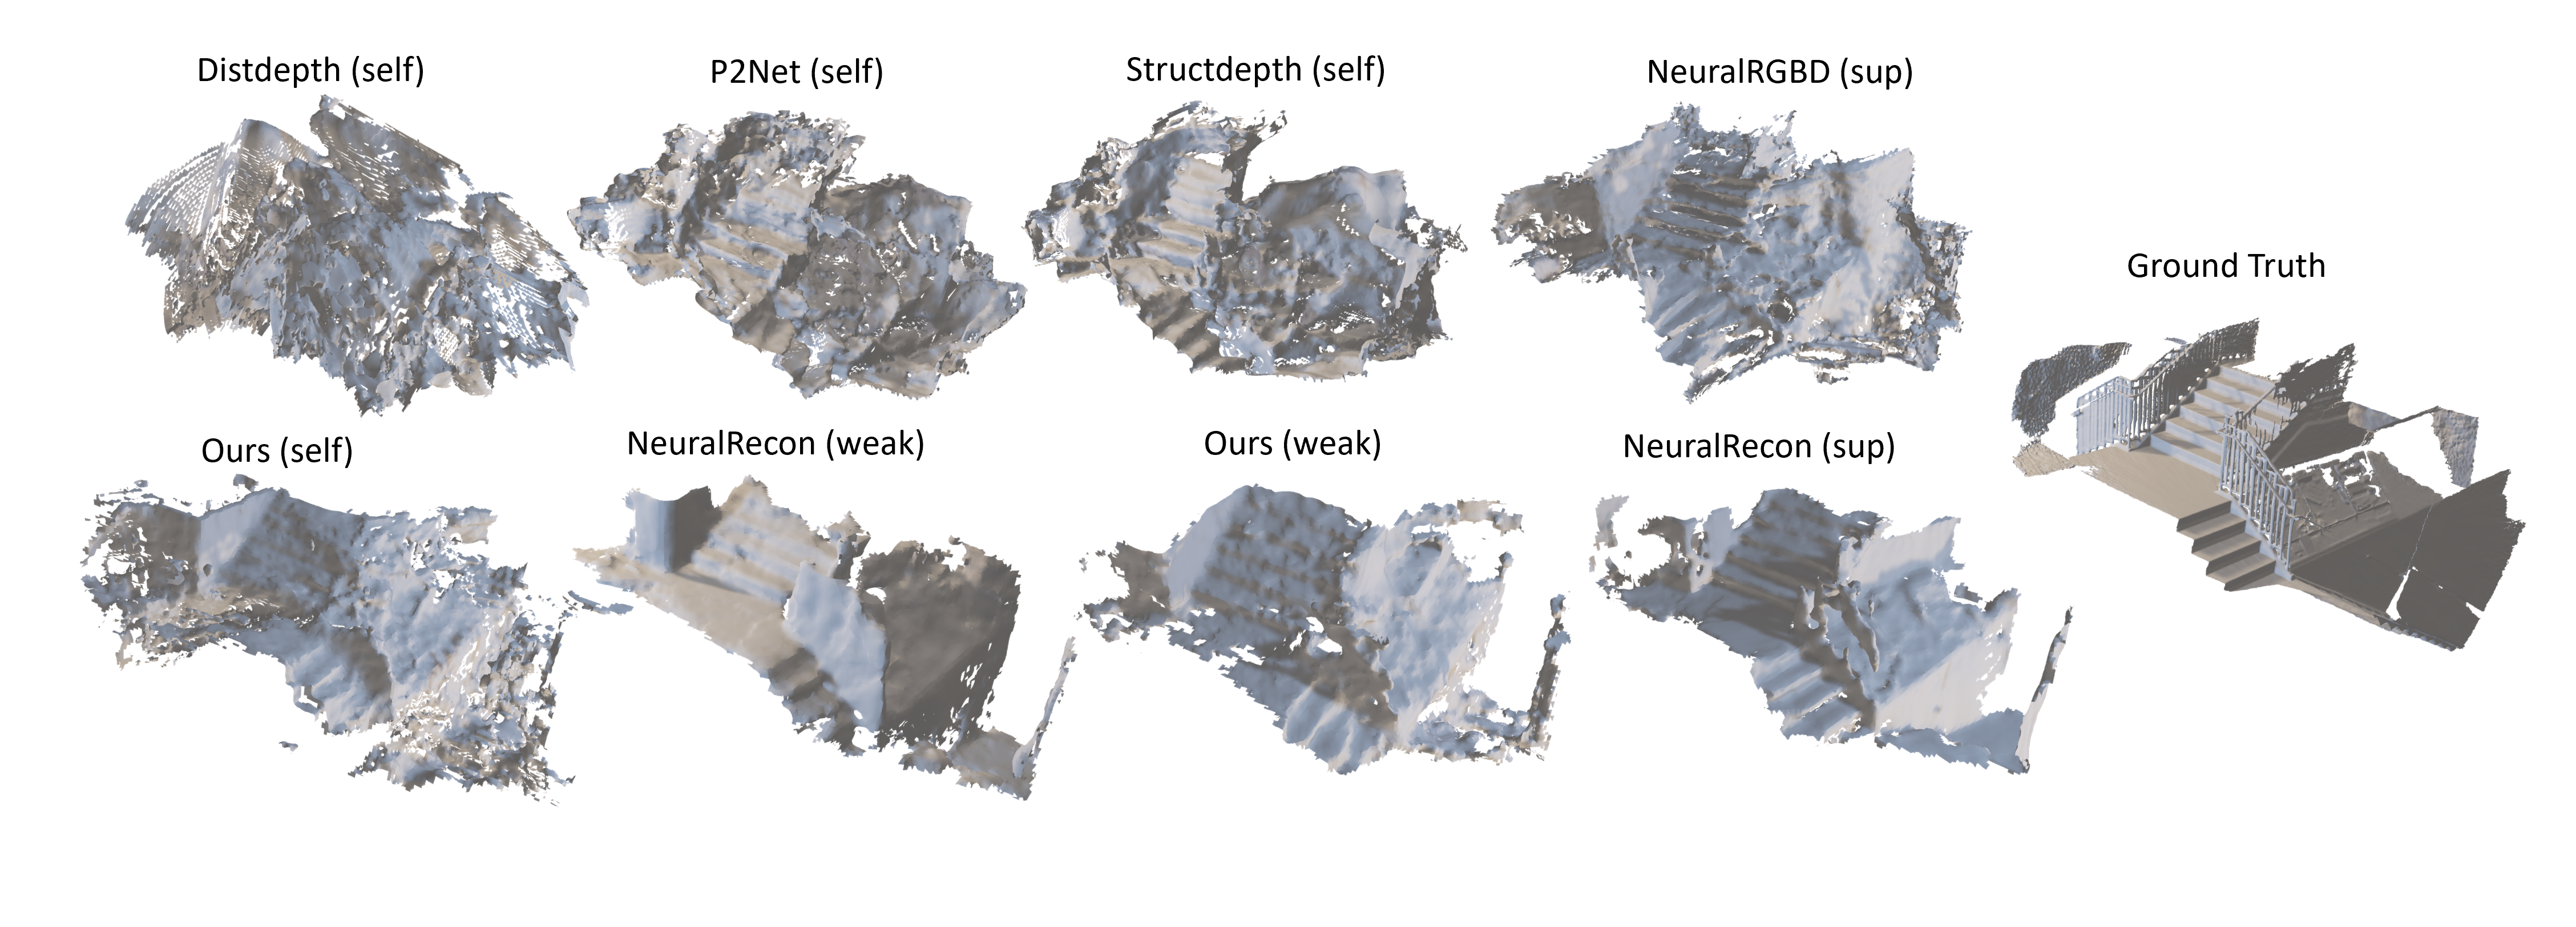
\includegraphics[width=1.0\textwidth]{figures/scannet_mesh/792.png}}
\end{minipage}
\vfill
\vspace{-8mm}
\begin{minipage}{\linewidth}
  \centerline{\includegraphics[width=1.0\textwidth]{figures/scannet_depth/738_1200.png}}
\end{minipage}

%\vspace{-3mm}
\begin{minipage}{\linewidth}
  \centerline{\includegraphics[width=1.0\textwidth]{figures/scannet_depth/747_1740.png}}
\end{minipage}
\vspace{-3mm}
\caption{\textbf{Visual Results on ScanNet.} 3D meshes are shown at top, 2D rendered depth maps are shown at bottom. Our self-supervised results are clearly better than SOTA self-supervised methods on challenging cases and fuzzy RGB input, even better than supervised depth estimation for a few cases. With weak supervision, our result is clearly better than NeuralRecon with weak supervision, which demonstrates our self-supervised design.}
\label{fig:visual results}
\end{figure*}